% =================================================================
\documentclass[ 10pt, xcolor = dvipsnames]{beamer}
\usepackage{ beamerthemesplit, lmodern}
\usetheme{Madrid}
\usecolortheme[named=Brown]{structure}
\useinnertheme{rectangles}
\setbeamertemplate{frametitle continuation}{}
\beamertemplatenavigationsymbolsempty
\usepackage{../../macros-general}
\usepackage{../../macros-beamer}
\graphicspath{{./figures/}}

\newcommand{\theoremblock}[2]{
\begin{center}
\begin{minipage}{0.9\columnwidth}
\begin{block}{#1}
#2
\end{block}
\end{minipage}
\end{center}
}

% =================================================================
\newcommand{\shorttitle}{Control Systems Engineering - Unit 03}
\title[\shorttitle]{Control Systems Engineering (EYAG-1005): \\ \textbf{Unit 03} }
\author[L. I. Reyes-Castro]{Luis I. Reyes-Castro}
\institute[ESPOL]{\normalsize Escuela Superior Polit\'ecnica del Litoral (ESPOL) \\ Guayaquil - Ecuador}
\date[2017-T1]{Semester: 2017-T1}

% -----------------------------------------------------------------
\begin{document}
\begin{frame}[noframenumbering]
\titlepage
\end{frame}
\begin{frame}[noframenumbering]
\frametitle{\shorttitle}
\tableofcontents[ subsectionstyle = hide]
\end{frame}

\AtBeginSection[]
{
\begin{frame}
\frametitle{Contenido del Tema}
\tableofcontents[ currentsection, sectionstyle = show/shaded, subsectionstyle = show/show/hide]
\end{frame}
}
\AtBeginSubsection[]
{
\begin{frame}
\frametitle{Contenido del Tema}
\tableofcontents[ currentsection, currentsubsection, sectionstyle = show/shaded, subsectionstyle = show/shaded/hide]
\end{frame}
}


%% =================================================================
%\section{First-order Systems}

%% =================================================================
%\section{Second-order Systems}

%% =================================================================
%\section{Stability}

% =================================================================
\section{Steady-state Errors}

% -----------------------------------------------------------------
\begin{frame}[allowframebreaks]
\frametitle{\insertsection}

Recall the reference signals: 
\begin{figure}
\centering
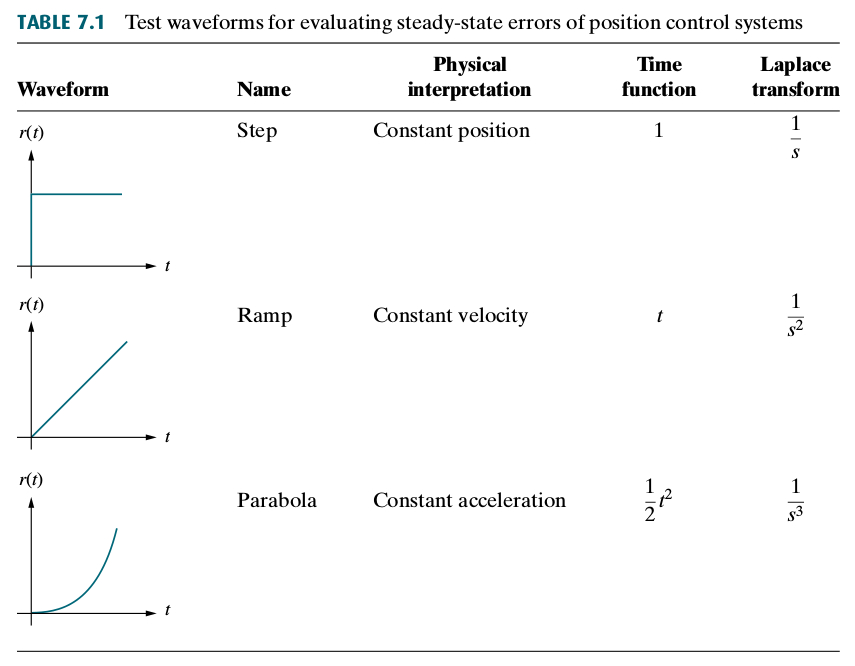
\includegraphics[width=0.72\columnwidth]{figures/Nise_Table-7-1.jpg}
\end{figure}
\framebreak

Recall the following result: 

\theoremblock{Laplace Transform - Final Value Theorem}{
For any function $f(t)$ defined for $t \geq 0$ with Laplace Transform $F(s)$ \linebreak we have that: 
\[
\lim_{ t \rightarrow \infty } \, f(t) \quad = \quad
\lim_{ s \rightarrow 0 } \, s \, F(s)
\]
\halfskip
}

\end{frame}

% -----------------------------------------------------------------
\begin{frame}[allowframebreaks]
\frametitle{\insertsection}

Steady-state errors for feedthrough systems: 
\fullskip

\begin{figure}
\centering
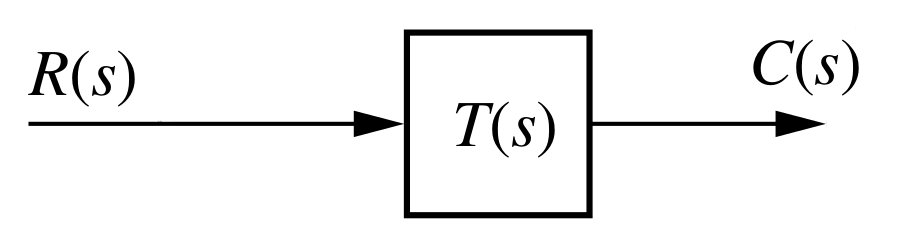
\includegraphics[width=0.4\columnwidth]{figures/Nise_Fig-7-3a.jpg}
\end{figure}
\begin{align*}
& E(s) \; = \; R(s) - C(s) \; = \; R(s) - T(s) \, R(s) \\[1ex]
& \Longrightarrow \; E(s) \; = \; R(s) \, [ \, 1 - T(s) \, ] \\[1ex]
& \Longrightarrow \; e(\infty) \; = \; 
\lim_{ t \rightarrow \infty } e(t) \; = \; 
\lim_{ s \rightarrow 0 } \; s \, R(s) \, [ \, 1 - T(s) \, ]
\end{align*}
\framebreak

\begin{itemize}
\item Step input $r(t) \, = \, u(t)$ :
\[
R(s) \, = \, \frac{1}{s} \qquad \Longrightarrow \qquad
e(\infty) \; = \; 
\lim_{ s \rightarrow 0 } \; 1 - T(s)
\]
\item Ramp input $r(t) \, = \, t \, u(t)$ :
\[
R(s) \, = \, \frac{1}{s^2} \qquad \Longrightarrow \qquad
e(\infty) \; = \; 
\lim_{ s \rightarrow 0 } \; \frac{1 - T(s)}{s}
\]
\item Parabolic input $r(t) \, = \, (1/2) \, t^2 \, u(t)$ :
\[
R(s) \, = \, \frac{1}{s^3} \qquad \Longrightarrow \qquad
e(\infty) \; = \; 
\lim_{ s \rightarrow 0 } \; \frac{1 - T(s)}{s^2}
\]
\end{itemize}

\end{frame}

% -----------------------------------------------------------------
\begin{frame}[allowframebreaks]
\frametitle{\insertsection}

Steady-state errors for unity-feedback systems: 
\fullskip

\begin{figure}
\centering
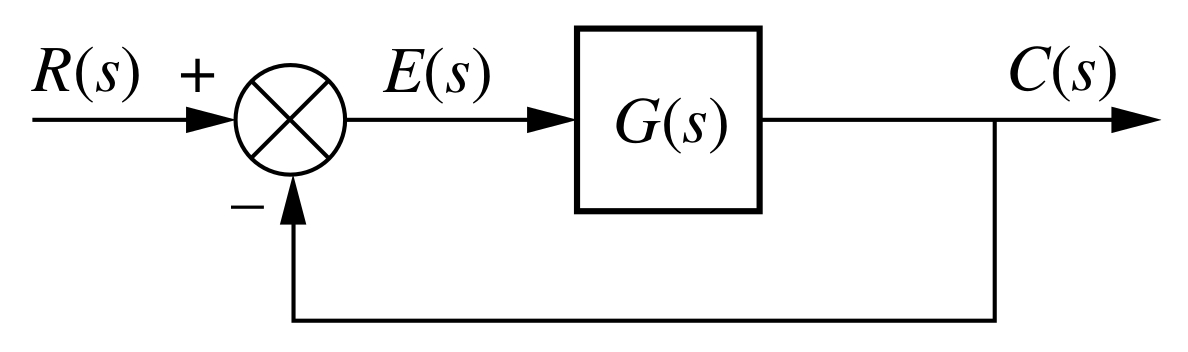
\includegraphics[width=0.5\columnwidth]{figures/Nise_Fig-7-3b.jpg}
\end{figure}
\begin{align*}
& E(s) \; = \; R(s) - C(s) \; = \; R(s) - G(s) \, E(s) \\[1ex]
& \Longrightarrow \; E(s) \, [ \, 1 + G(s) \, ] \; = \; R(s) \\[1ex]
& \Longrightarrow \; E(s) \; = \; \frac{R(s)}{1 + G(s)} \\[1ex]
& \Longrightarrow \; e(\infty) \; = \; 
\lim_{ t \rightarrow \infty } e(t) \; = \; 
\lim_{ s \rightarrow 0 } \; \frac{ s \, R(s) }{1 + G(s)}
\end{align*}
\framebreak

\begin{itemize}
\item Step input $r(t) \, = \, u(t)$ :
\[
R(s) \, = \, \frac{1}{s} \qquad \Longrightarrow \qquad
e_{step}(\infty) \; = \; 
\lim_{ s \rightarrow 0 } \; \frac{1}{1 + G(s)}
\]
\item Ramp input $r(t) \, = \, t \, u(t)$ :
\[
R(s) \, = \, \frac{1}{s^2} \qquad \Longrightarrow \qquad
e_{ramp}(\infty) \; = \; 
\lim_{ s \rightarrow 0 } \; \frac{1}{s \, G(s)}
\]
\item Parabolic input $r(t) \, = \, (1/2) \, t^2 \, u(t)$ :
\[
R(s) \, = \, \frac{1}{s^3} \qquad \Longrightarrow \qquad
e_{parabolic}(\infty) \; = \; 
\lim_{ s \rightarrow 0 } \; \frac{1}{s^2 \, G(s)}
\]
\end{itemize}

\end{frame}

% -----------------------------------------------------------------
\begin{frame}[allowframebreaks]
\frametitle{\insertsection}

Furthermore, for unity-feedback systems: 
\begin{itemize}
\item Position constant $K_p$ :
\[
K_p \; = \; \lim_{ s \rightarrow 0 } \; G(s)
\qquad \Longrightarrow \qquad
e_{step}(\infty) \; = \; \frac{1}{1 + K_p}
\]
\item Velocity constant $K_v$ :
\[
K_v \; = \; \lim_{ s \rightarrow 0 } \; s \,G(s)
\qquad \Longrightarrow \qquad
e_{ramp}(\infty) \; = \; \frac{1}{K_v}
\]
\item Acceleration constant $K_a$ :
\[
K_a \; = \; \lim_{ s \rightarrow 0 } \; s^2 \,G(s)
\qquad \Longrightarrow \qquad
e_{ramp}(\infty) \; = \; \frac{1}{K_a}
\]
\end{itemize}

\end{frame}

% -----------------------------------------------------------------
\begin{frame}[allowframebreaks]
\frametitle{\insertsection}

For non-unity non-unity-feedback systems, simply re-write the system in unity-feedback form: 
\fullskip

\begin{figure}
\centering
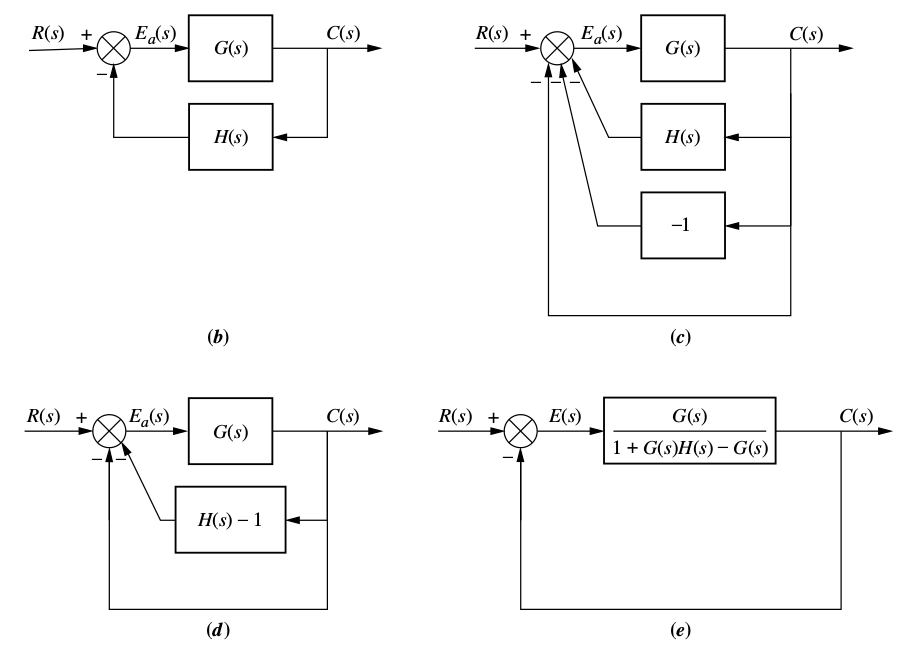
\includegraphics[width=0.7\columnwidth]{figures/Nise_Fig-7-15.jpg}
\end{figure}

\end{frame}

\end{document}
